\begin{dang}{Xác định góc và tính tích vô hướng của hai véctơ}
\end{dang}
\boxmini{BÀI TẬP TỰ LUẬN}
\setcounter{vd}{0}
\begin{vd}
	Cho hình lập phương $ ABCD.A'B'C'D' $ có cạnh bằng 5.
	\begin{tasks}
	\task Tìm góc giữa các cặp véc-tơ sau: $\vec{AC}$ và $\vec{AB}$; $\vec{AC}$ và $\vec{B'D'}$; $\vec{AC}$ và $\vec{CD}$; $\vec{AD'}$ và $\vec{BD}$.
	\task Tính các tích vô hướng $\vec{AC}\cdot \vec{AB}$; $\vec{AC}\cdot \vec{B'D'}$; $\vec{AD'}\cdot\vec{BD}$;
	\task Chứng minh $\vec{AC'}$ vuông góc với $\vec{BD}$.
	\end{tasks}
	\loigiai{
	\immini{\begin{enumerate}[a)]
	\item Ta có :
	 \begin{itemize}
	 \item [$\bullet$] $\left( \vec{AC},\vec{AB}\right)=\widehat{CAB}=45^\circ$
	 \item [$\bullet$] $\left(\vec{AC},\vec{B'D'}\right)=\left(\vec{AC},\vec{BD}\right)=90^\circ$.
	 \item [$\bullet$] $\left(\vec{AC},\vec{CD}\right)=\left(\vec{CE},\vec{CD}\right)=180^\circ-45^\circ=135^\circ$ (E là điểm đối xứng của $A$ qua $C$).
	 \item [$\bullet$] $ \vec{AD'}=\vec{BC'} \Rightarrow \left(\vec{AD'},\vec{BD}\right)=\left(\vec{BC'},\vec{BD}\right)=\widehat{C'BD}$.
	 Lại có, tam giác $ C'BD $ là tam giác đều nên $ \widehat{C'BD}=60^\circ\Rightarrow \left(\vec{AD'},\vec{BD}\right)=60^\circ $.
	 \end{itemize}
	\item Ta có $AC=BD=B'D'=5\sqrt{2}$. Suy ra
	 \begin{itemize}
	 \item [$\bullet$] $\vec{AC}\cdot \vec{AB}=AC.AB.\cos45^\circ =25$.
	 \item [$\bullet$] Do $AC$ vuông góc $B'D'$ nên $\vec{AC}\cdot \vec{B'D'}=0$.
	 \item [$\bullet$] $\vec{AD'}\cdot \vec{BD}=AD'.BD.\cos60^\circ =5\sqrt{2}.5\sqrt{2}.\dfrac{1}{2}=25$.
	 \end{itemize}
	\item Ta cần chứng minh $\vec{AC'}\cdot \vec{BD}=0$.\\
	 Ta có: $\vec{AC'}=\vec{AB}+\vec{AD}+\vec{AA'}$ và $\vec{BD}=\vec{AD}-\vec{AB}$ nên
	 \begin{eqnarray*}
	 \vec{AC'}\cdot \vec{BD}
	 &=&\left( \vec{AB}+\vec{AD}+\vec{AA'}\right)\cdot \left(\vec{AD}-\vec{AB} \right) \\
	 &=&\vec{AB}.\vec{AD}-\vec{AB}^2+\vec{AD}^2-\vec{AD}.\vec{AB}+\vec{AA'}.\vec{AD}-\vec{AA'}.\vec{AB}=5^2-5^2=0
	 \end{eqnarray*}
	 Suy ra $\vec{AC'}$ vuông góc với $\vec{BD}$.
	\end{enumerate}}{
	\begin{tikzpicture}[scale=0.6, font=\footnotesize, line join=round, line cap=round]
	\def\h{4}
	\foreach \x\y\t in {0/0/A,-1/-1.1/B,2.6/-1.1/C}
	\coordinate (\t) at (\x,\y);
	\coordinate (D) at ($(A)+(C)-(B)$);
	\coordinate (A') at ($(A)+(0,3.2)$);
	\coordinate (B') at ($(B)+(0,3.2)$);
	\coordinate (C') at ($(C)+(0,3.2)$);
	\coordinate (D') at ($(D)+(0,3.2)$);
	\coordinate (E) at ($2*(C)-(A)$);
	\draw (B')--(A')--(D')--(C')--(B')--(B)--(C)--(D)--(D') (C')--(C)--(E);
	\draw[dashed](B)--(A)--(D) (A)--(A') (A)--(C);
	\foreach \t/\g in {A/170,B/-150,C/-100,D/0,A'/100,B'/170,C'/-20,D'/50,E/0}
	\draw[fill=black] (\t) circle(1pt)
	node[shift={(\g:7pt)}]{$\t$};
	\end{tikzpicture}
	}
	}
\end{vd}

\begin{vd}%[2H2H1-3]
	Cho tứ diện đều $ABCD$ có cạnh bằng $a$ và $M$ là trung điểm của $CD$.
	\begin{listEX}[2]
	\item Tính các tích vô hướng $\vec{AB} \cdot \vec{AC}$, $\vec{AB} \cdot \vec{AM}$.
	\item Tính góc $(\vec{AB}, \vec{CD})$.
	\end{listEX}
	\loigiai{
	\begin{enumerate}
	\item Ta có $\begin{aligned}[t]
	 \vec{AC} \cdot \vec{AC} & = |\vec{AB}| \cdot |\vec{AC}| \cdot \cos (\vec{AB},\vec{AC}) \\
	 & = AB \cdot AC \cdot \cos \widehat{BAC} \\
	 & = a \cdot a \cdot \cos {60^0} \\
	 & = \frac{a^2}{2}.
	 \end{aligned}$\\
	 Tương tự ta cũng có $\vec{AB} \cdot \vec{AD} = \dfrac{a^2}{2}$.
	 \immini{
	 Ta lại có $\vec{AM} = \dfrac{1}{2}(\vec{AC} + \vec{AD})$, suy ra
	 \[ \vec{AB} \cdot \vec{AM} = \vec{AB} \cdot \frac{1}{2}(\vec{AC} +\vec{AD}) = \frac{1}{2}(\vec{AB} \cdot \vec{AC} + \vec{AB} \cdot \vec{AD}) = \frac{1}{2}\left(\frac{a^2}{2} + \frac{a^2}{2}\right) = \frac{a^2}{2}.\]
	\item Ta có $\vec{AB} \cdot \vec{CD}=(\vec{AM}+\vec{MB}) \cdot \vec{CD}=\vec{AM} \cdot \vec{CD} +\vec{MB} \cdot \vec{CD}$.\\
	 Mà $AM$, $BM$ là trung tuyến của các tam giác đều $ACD$, $BCD$ nên $\vec{AM} \perp \vec{CD}, \vec{MB} \perp \vec{CD}$.\\
	 Suy ra $\vec{AM} \cdot \vec{CD} = \vec{MB} \cdot \vec{CD} = 0$.\\
	 Từ các kết quả trên ta có $\vec{AM} \cdot \vec{CD}=0$.
	 Suy ra $(\vec{AB}, \vec{CD})=90^\circ$.
	 }{
	 \begin{tikzpicture}[scale=1, font=\footnotesize, line join=round, line cap=round, >=Stealth]
	 \def\a{3}
	 \path
	 (0:0) coordinate (B)
	 (5:\a) coordinate (D)
	 ($(D)+(-135:\a/2)$) coordinate (C)
	 ($(B)+(65:\a)$) coordinate (A)
	 ($(C)!.5!(D)$) coordinate (M)
	 ;
	 \draw[->] (A)--(D);
	 \draw[->] (A)--(C);
	 \draw[->] (A)--(B);
	 \draw[->] (A)--(M);
	 \draw[dashed] (B)--(D);
	 \draw (B)--(C)--(D);
	 \foreach \x/\g in {A/90,B/180,C/-90,D/0,M/0}
	 \draw[fill=black] 	(\x) circle (.5pt)
	 ($(\g:.3)+(\x)$) node {$\x$};
	 \end{tikzpicture}
	 }
	\end{enumerate}
	}
\end{vd}

\begin{vd}
	\immini{Cho biết công $A$ (đơn vị: $J$) sinh bởi lực $\vec{F}$ tác dụng lên một vật được tính bằng công thức $A = \vec{F}\cdot\vec{d}$, trong đó $\vec{d}$ là vectơ biểu thị độ dịch chuyển của vật (đơn vị của $\left|\vec{d}\right|$ là m) khi chịu tác dụng của lực $\vec{F}$.
	}{
	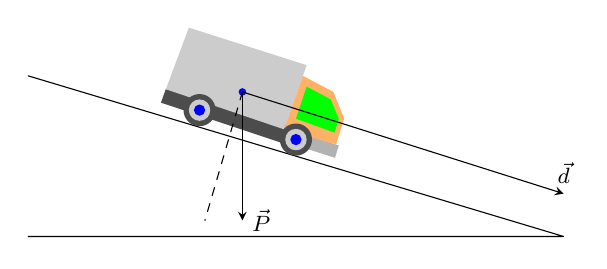
\begin{tikzpicture}[scale=0.68,font=\footnotesize, line join=round, line cap=round, >=stealth]
	\def\xe{orange!60}
	\def\den{red}
	\draw (0,3)--(10,0) (0,0)--(10,0);
	\fill[black!30] (2.48,2.5)--(2.57,2.75)--(5.8,1.7)--(5.73,1.47)--cycle ;
	\fill[black!70] (2.48,2.5)--(2.57,2.75)--(5.2,2)--(5.18,1.6)--cycle ;
	\fill[black!20] (2.57,2.75)--(3,3.9)--(5.2,3.2)--(4.78,2)--cycle ;
	\fill[\xe] (4.78,2)--(5.13,3)--(5.7,2.7)--(5.9,2.2)--(5.75,1.72)--cycle ;
	\fill[green] (5.2,2.8)--(5.65,2.56)--(5.8,2.2)--(5.72,1.94)--(5,2.2)--cycle ;
	\fill[black!70] (3.2,2.36) circle (0.3) (5,1.81) circle (0.3) ;
	\fill[black!20] (3.2,2.36) circle (0.2) (5,1.81) circle (0.2) ;
	\fill[blue](3.2,2.36) circle (3pt) (5,1.81) circle (3pt) (4,2.7) circle (2pt) ;
	\draw[dashed] (4,2.7)--(3.3,0.3) ;
	\draw[->] (4,2.7)--(4,0.3) node[right] {$\vec{P}$};
	\draw[->] (4,2.7)--(10,0.8) node[above] {$\vec{d}$};
	\end{tikzpicture} }
	Một chiếc xe có khối lượng $1{,}5$ tấn đang đi xuống trên một đoạn đường dốc có góc nghiêng $5^\circ$ so với phương ngang. Tính công sinh bởi trọng lực $\vec{P}$ khi xe đi hết đoạn đường dốc dài $30$ m (làm tròn kết quả đến hàng đơn vị), biết rằng trọng lực $\vec{P}$ được xác định bởi công thức $\vec{P} = m\vec{g}$, với $m$ (đơn vị: kg) là khối lượng của vật và $\vec{g}$ là gia tốc rơi tự do có độ lớn $g = 9{,}8$ m/s$^2$.
	\loigiai{
	\begin{center}
	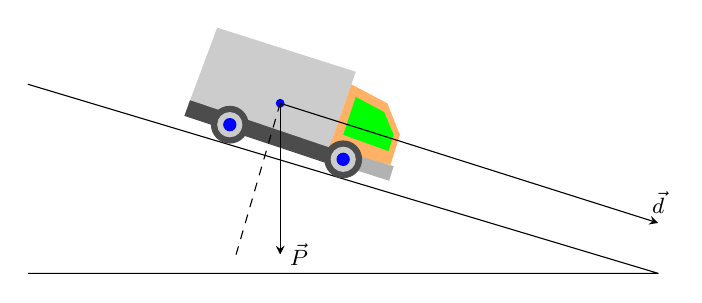
\begin{tikzpicture}[scale=0.8,font=\footnotesize, line join=round, line cap=round, >=stealth]
	\def\xe{orange!60}
	\def\den{red}
	\draw (0,3)--(10,0) (0,0)--(10,0);
	\fill[black!30] (2.48,2.5)--(2.57,2.75)--(5.8,1.7)--(5.73,1.47)--cycle ;
	\fill[black!70] (2.48,2.5)--(2.57,2.75)--(5.2,2)--(5.18,1.6)--cycle ;
	\fill[black!20] (2.57,2.75)--(3,3.9)--(5.2,3.2)--(4.78,2)--cycle ;
	\fill[\xe] (4.78,2)--(5.13,3)--(5.7,2.7)--(5.9,2.2)--(5.75,1.72)--cycle ;
	\fill[green] (5.2,2.8)--(5.65,2.56)--(5.8,2.2)--(5.72,1.94)--(5,2.2)--cycle ;
	\fill[black!70] (3.2,2.36) circle (0.3) (5,1.81) circle (0.3) ;
	\fill[black!20] (3.2,2.36) circle (0.2) (5,1.81) circle (0.2) ;
	\fill[blue](3.2,2.36) circle (3pt) (5,1.81) circle (3pt) (4,2.7) circle (2pt) ;
	\draw[dashed] (4,2.7)--(3.3,0.3) ;
	\draw[->] (4,2.7)--(4,0.3) node[right] {$\vec{P}$};
	\draw[->] (4,2.7)--(10,0.8) node[above] {$\vec{d}$};
	\end{tikzpicture}
	%\includegraphics{hinhanh/H1.png} 
	\end{center}
	\noindent
	Ta có $1{,}5$ tấn = $1~500$ kg.\\
	Độ lớn của trọng lực tác dụng lên chiếc xe là $\left|\vec{P}\right| = m \left|\vec{g}\right| = 1~500\cdot 9{,}8 = 14~700$ (N).\\
	Vectơ d biểu thị độ dịch chuyển của xe có độ dài là $\left|\vec{d}\right| = 30$ (m) và $ \left(\vec{P},\vec{d}\right)= 90^\circ - 5^\circ = 85^\circ$.\\
	Công sinh ra bởi trọng lực $\vec{P}$ khi xe đi hết đoạn đường dốc dài $30$ m là
	$$A=\vec{P}\cdot\vec{d}=\left|\vec{P}\right|\cdot\left|\vec{d}\right|\cdot\cos\left(\vec{P},\vec{d}\right) = 14~700\cdot 30\cdot \cos 85^\circ \approx 38~436~(J).$$
	}
\end{vd}

\begin{vd}
	\immini{
	Một chất điểm $A$ nằm trên mặt phẳng nằm ngang $\left(\alpha\right)$, chịu tác động bởi ba lực $\vec{F}_1$, $\vec{F}_2$, $\vec{F}_3$. Các lực $\vec{F}_1$, $\vec{F}_2$ có giá nằm trong $\left(\alpha\right)$ và $\left(\vec{F}_1, \vec{F}_2\right)=135^\circ$, còn lực $\vec{F}_3$ có giá vuông góc với $\left(\alpha\right)$ và hướng lên trên. Xác định cường độ hợp lực của các lực $\vec{F}_1$, $\vec{F}_2$, $\vec{F}_3$ biết rằng độ lớn của ba lực đó lần lượt là $20$ N, $15$ N và $10$ N.
	}{
	\begin{tikzpicture}[line join=round, line cap = round, >=stealth, scale=0.75,font=\footnotesize]
	\path
	(0,0) coordinate (A)
	(-2,-1.5) coordinate (B)
	(3,0) coordinate (C)
	(0,3) coordinate (D)
	;
	\draw[->] (A)--(B) node[below] {$\vec{F}_1$};
	\draw[->] (A)--(C) node[below] {$\vec{F}_2$};
	\draw[->] (A)--(D) node[right] {$\vec{F}_3$};
	\draw pic[draw,angle eccentricity=1.2,angle radius=0.2cm]{right angle= D--A--C};
	\draw pic[draw,angle eccentricity=1.2,angle radius=0.2cm]{right angle= D--A--B};
	\draw pic[draw,angle eccentricity=1.2,angle radius=0.3cm]{angle= B--A--C};
	\draw ($(A)-(-0.3,0.6)$) node {$135^\circ$};
	\foreach \x/\g in {A/140} \fill[black](\x) circle (1pt) ($(\x)+(\g:4mm)$)node{$\x$};
	\end{tikzpicture}
	}
	\loigiai{
	Gọi $\vec{F}$ là hợp lực của các lực $\vec{F}_1$, $\vec{F}_2$, $\vec{F}_3$, tức là $\vec{F}= \vec{F}_1+ \vec{F}_2+ \vec{F}_3$, ta có
	\allowdisplaybreaks
	\begin{eqnarray*}
	\left|\vec{F}\right|^2 &=& \left(\vec{F}_1+ \vec{F}_2+ \vec{F}_3\right)^2\\
	&=& \vec{F}_1^2+ \vec{F}_2^2+ \vec{F}_3^2+ 2\vec{F}_1\cdot\vec{F}_2+ 2\vec{F}_2\cdot\vec{F}_3+ 2\vec{F}_3\cdot\vec{F}_1\\
	&=& 20^2+ 15^2+ 10^2+ 2\cdot 20\cdot 15\cdot\cos 135^\circ\\
	&=& 725-300\sqrt2.
	\end{eqnarray*}
	Vậy $\left|\vec{F}\right|= \sqrt{725-300\sqrt2} \approx 17{,}34$ (N).
	}
\end{vd}

\boxmini{BÀI TẬP TRẮC NGHIỆM}
\textbf{PHẦN I.} \textit{Câu trắc nghiệm nhiều phương án lựa chọn. Mỗi câu hỏi học sinh chỉ chọn một phương án.}\\
\setcounter{ex}{0}
\Opensolutionfile{ans}[ans/2H2-B1-d2-1]
%%==========Câu 1
\begin{ex}
	\immini{Cho hình lập phương $ABCD.A'B'C'D'$. Khẳng định nào sau đây là khẳng định \textbf{sai}?
	\choice
	{ $\left(\vec{A'C'},\vec{AD}\right)=45^\circ$}
	{$\left(\vec{A'C'},\vec{B'B}\right)=90^\circ$}
	{\True $\left(\vec{A'A}, \vec{CB'}\right)=45^\circ$}
	{$\left(\vec{AB},\vec{CD}\right)=180^\circ$}
	}{
	\begin{tikzpicture}[scale=0.65, font=\footnotesize,>=stealth]
	%Gán số liệu.
	\def\canhAD{3};\def\canhBA{2};\def\gocBAD{-130};\def\h{3};\def\xdinhA'{0};
	%Gán tọa độ.
	\coordinate (A) at (0,0);
	\coordinate (B) at ($(A)+(\gocBAD:\canhBA)$);
	\coordinate (C) at ($(B)+(0:\canhAD)$);
	\coordinate (D) at ($(A)+(0:\canhAD)$);
	\coordinate (A') at ($(A)+(\xdinhA',\h)$);
	\coordinate (B') at ($(B)+(\xdinhA',\h)$);
	\coordinate (C') at ($(C)+(\xdinhA',\h)$);
	\coordinate (D') at ($(D)+(\xdinhA',\h)$);
	%Vẽ khối lẳng trụ ABCD.A'B'C'D'.
	\draw (A')--(B')--(B)--(C)--(C')--(D')--cycle (B')--(C') (D')--(D)--(C) (A')--(C');
	\draw[dashed] (A)--(D) (A')--(A)--(B) (A)--(C);
	%Gán nhãn.
	\foreach \x/\y in {A/180, B/180, C/0, D/0, A'/180, B'/180, C'/0, D'/0}{\fill (\x) circle(1pt) ($(\x)+(\y:0.3cm)$) node{$\x$};}
	\end{tikzpicture}}
	\loigiai{
	\begin{itemize}
	\item [$\bullet$] Ta có $\left(\vec{A'C'},\vec{AD}\right)=\left(\vec{A'C'},\vec{A'D'}\right)=\widehat{C'A'D'}=45^\circ$.
	\item [$\bullet$] $\left(\vec{A'C'},\vec{B'B}\right)=\left(\vec{A'C'},\vec{A'A}\right)=\widehat{AA'C'}=90^\circ$.
	\item [$\bullet$] Ta có $\vec{B'B}=\vec{A'A}$, suy ra\\
	 $\left(\vec{A'A},\vec{CB'}\right)=\left(\vec{B'B},\vec{CB'}\right)=180^{\circ}-\widehat{BB'C}=180^{\circ}-45^{\circ}=135^{\circ}$
	\item [$\bullet$] $\vec{AB}$ ngược hướng với $\vec{CD}$ nên $\left(\vec{AB},\vec{CD}\right)=180^\circ$.
	\end{itemize}
	}
\end{ex} 
%%==========Câu 2
\begin{ex}
	\immini{Cho tứ diện đều $ABCD$, Gọi $M$, $N$ lần lượt là trung điểm các cạnh $AB$, $AC$. Hãy tính góc giữa hai vectơ $\vec{MN}$ và $\vec{BD}$.
	\choice
	{$ \left(\vec{MN}, \vec{BD} \right) = 150^\circ$}
	{$ \left(\vec{MN}, \vec{BD} \right) = 120^\circ$}
	{$ \left(\vec{MN}, \vec{BD} \right) = 30^\circ$}
	{\True $ \left(\vec{MN}, \vec{BD} \right) = 60^\circ$}}{
	\begin{tikzpicture}[scale=0.55, font=\footnotesize, line join=round, line cap=round]
	\foreach \x\y\t in {0/0/B,6/0/D,1.5/-2/C,1.5/5/A}
	\coordinate (\t) at (\x,\y);
	\coordinate (M) at ($(A)!1/2!(B)$);
	\coordinate (N) at ($(A)!1/2!(C)$);
	\draw (A)--(B)--(C)--(D)--(A)--(C) (M)--(N);
	\draw[dashed] (B)--(D);
	\foreach \t/\g in {A/90,B/180,C/-90,D/0,M/180,N/0} \draw (\t) node[shift={(\g:10pt)}]{$\t$};
	\end{tikzpicture}}
	\loigiai{
	\immini{Xét tam giác $ABC$ có $M$, $N$ là trung điểm của $AB$, $AC$ nên $MN$ là đường trung bình của tam giác $ABC$. Do đó $MN \parallel BC$.\\
	Ta có $ \left(\vec{MN}, \vec{BD} \right)= \left(\vec{BC}, \vec{BD} \right) = \widehat{CBD}$. \\
	Vì $ABCD$ là tứ diện đều nên $BC=CD=DB$. Do đó tam giác $BCD$ đều suy ra $\widehat{CBD} = 60^\circ$.\\
	Vậy $ \left(\vec{MN}, \vec{BD} \right) = 60^\circ$.}
	{\begin{tikzpicture}[scale=0.55, font=\footnotesize, line join=round, line cap=round]
	\foreach \x\y\t in {0/0/B,6/0/D,1.5/-2/C,1.5/5/A}
	\coordinate (\t) at (\x,\y);
	\coordinate (M) at ($(A)!1/2!(B)$);
	\coordinate (N) at ($(A)!1/2!(C)$);
	\draw (A)--(B)--(C)--(D)--(A)--(C);
	\draw[dashed,-stealth,blue,very thick] (B)--(D);
	\draw[-stealth,blue,very thick](M)--(N);
	\foreach \t/\g in {A/90,B/180,C/-90,D/0,M/180,N/0} \draw (\t) node[shift={(\g:10pt)}]{$\t$};
	\end{tikzpicture}}
	}
\end{ex} 
%%==========Câu 3
\begin{ex}
	\immini{Cho hình chóp $S. A B C D$ có đáy $A B C D$ là hình bình hành và mặt bên $S A B$ là tam giác đều. Tính góc giữa hai vectơ $\vec{D C}$ và $\vec{B S}$.
	\haicot
	{\True $\left(\vec{D C}, \vec{B S}\right)=120^{\circ}$}
	{$\left(\vec{D C}, \vec{B S}\right)=60^{\circ}$}
	{$\left(\vec{D C}, \vec{B S}\right)=90^{\circ}$}
	{$\left(\vec{D C}, \vec{B S}\right)=150^{\circ}$}
	}{
	\begin{tikzpicture}[scale=0.8, font=\footnotesize,>=stealth]
	%Gán số liệu.
	\def\canhAD{4};\def\canhBA{2};\def\gocBAD{-130};\def\h{2};\def\xdinhS{-1};
	%Gán tọa độ.
	\coordinate (A) at (0,0);
	\coordinate (B) at ($(A)+(\gocBAD:\canhBA)$);
	\coordinate (C) at ($(B)+(0:\canhAD)$);
	\coordinate (D) at ($(A)+(0:\canhAD)$);
	\coordinate (S) at ($(A)+(\xdinhS,\h)$);
	\draw (B)--(S)--(C)--cycle (S)--(D)--(C);
	\draw[dashed] (A)--(D) (S)--(A)--(B);
	\foreach \x/\y in {A/180,B/-90,C/-90,D/0,S/90}{\fill (\x) circle(1pt) ($(\x)+(\y:0.3cm)$) node{$\x$};}
	\end{tikzpicture}
	}
	\loigiai{
	\immini{Vì $A B C D$ là hình bình hành nên $A B \parallel D C$.\\
	Trên tia $A B$ lấy điểm $E$ sao cho $\vec{B E}=\vec{D C}$ (Hình $2.20$). Ta có
	$$
	\left(\vec{D C}, \vec{B S}\right)=\left(\vec{B E}, \vec{B S}\right)=\widehat{E B S}=180^{\circ}-60^{\circ}=120^{\circ}.
	$$
	Vậy $\left(\vec{D C}, \vec{B S}\right)=120^{\circ}$.
	}{
	\begin{tikzpicture}[scale=0.8, font=\footnotesize,>=stealth]
	%Gán số liệu.
	\def\canhAD{4};\def\canhBA{2};\def\gocBAD{-130};\def\h{2};\def\xdinhS{-1};
	%Gán tọa độ.
	\coordinate (A) at (0,0);
	\coordinate (B) at ($(A)+(\gocBAD:\canhBA)$);
	\coordinate (C) at ($(B)+(0:\canhAD)$);
	\coordinate (D) at ($(A)+(0:\canhAD)$);
	\coordinate (S) at ($(A)+(\xdinhS,\h)$);
	\coordinate (E) at ($(B)!-1!(A)$);
	%Vẽ khối chóp S.ABCD.
	\draw (B)--(S)--(C)--cycle (S)--(D)--(C);
	\draw[dashed] (A)--(D) (S)--(A)--(B);
	\draw[->] (B)--(E);
	\draw[->] (D)--(C);
	%	%Gán nhãn.
	\draw pic["$60^\circ$",draw,angle eccentricity=1.6,angle radius=0.5cm]{angle=A--B--S};
	\draw pic["$120^\circ$",draw,double,angle eccentricity=1.7,angle radius=0.4cm]{angle=S--B--E};
	\foreach \x/\y in {A/180,B/-90,C/-90,D/0,S/90, E/90}{\fill (\x) circle(1pt) ($(\x)+(\y:0.3cm)$) node{$\x$};}
	\end{tikzpicture}
	}
	}
\end{ex} 
%%==========Câu 4
\begin{ex}
	\immini{Cho hình chóp $S.A B C D$ có đáy $A B C D$ là hình bình hành. Mặt bên $A S B$ là tam giác vuông cân tại $S$ và có cạnh $A B=a$. Tính $\vec{D C} \cdot \vec{A S}$.
	\haicot
	{$\dfrac{a^2}{4}$}
	{$-\dfrac{a^2}{4}$}
	{$-\dfrac{a^2}{2}$}
	{\True $\dfrac{a^2}{2}$}}{
	\begin{tikzpicture}[scale=0.79, font=\footnotesize,>=stealth]
	\def\canhAD{4};\def\canhBA{2};\def\gocBAD{-130};\def\h{2};\def\xdinhS{-1};
	%Gán tọa độ.
	\coordinate (A) at (0,0);
	\coordinate (B) at ($(A)+(\gocBAD:\canhBA)$);
	\coordinate (C) at ($(B)+(0:\canhAD)$);
	\coordinate (D) at ($(A)+(0:\canhAD)$);
	\coordinate (S) at ($(A)+(\xdinhS,\h)$);
	\draw (B)--(S)--(C)--cycle (S)--(D)--(C);
	\draw[dashed] (A)--(D) (S)--(A)--(B);
	\draw[->] (D)--(C);
	%\draw pic["$45^\circ$",draw,angle eccentricity=1.6,angle radius=0.3cm]{angle=S--A--B};
	\foreach \x/\y in {A/60,B/-90,C/-90,D/0,S/90}{\fill (\x) circle(1pt) ($(\x)+(\y:0.3cm)$) node{$\x$};}
	\end{tikzpicture}}
	\loigiai{
	\immini{$\vec{D C} \cdot \vec{A S}=\vec{A B} \cdot \vec{A S}=\left|\vec{A B}\right| \cdot\left|\vec{A S}\right| \cdot \cos \left(\vec{A B}, \vec{A S}\right)=a \cdot \dfrac{a \sqrt{2}}{2} \cdot \cos 45^{\circ}=\dfrac{a^2}{2}$.
	}{
	\begin{tikzpicture}[scale=0.9, font=\footnotesize,>=stealth]
	\def\canhAD{4};\def\canhBA{2};\def\gocBAD{-130};\def\h{2};\def\xdinhS{-1};
	%Gán tọa độ.
	\coordinate (A) at (0,0);
	\coordinate (B) at ($(A)+(\gocBAD:\canhBA)$);
	\coordinate (C) at ($(B)+(0:\canhAD)$);
	\coordinate (D) at ($(A)+(0:\canhAD)$);
	\coordinate (S) at ($(A)+(\xdinhS,\h)$);
	\draw (B)--(S)--(C)--cycle (S)--(D)--(C);
	\draw[dashed] (A)--(D) (S)--(A)--(B);
	\draw[->] (D)--(C);
	\draw pic["$45^\circ$",draw,angle eccentricity=1.6,angle radius=0.3cm]{angle=S--A--B};
	\foreach \x/\y in {A/60,B/-90,C/-90,D/0,S/90}{\fill (\x) circle(1pt) ($(\x)+(\y:0.3cm)$) node{$\x$};}
	\end{tikzpicture}}
	}
\end{ex} 
%%==========Câu 5
\begin{ex}
	\immini{Cho hình lập phương $ABCD.EFGH$ có các cạnh bằng $ a $. Tính $\vec{AB}\cdot\vec{EG}$.
	\haicot
	{$a^2\sqrt{2}$}
	{\True $a^2$}
	{$\dfrac{a^2\sqrt{2}}{2}$}
	{$a^2\sqrt{3}$}}{
	\begin{tikzpicture}[scale=0.5, font=\footnotesize, line join=round, line cap=round, >=stealth]
	\coordinate (A) at (0,0);
	\coordinate (B) at (-1.5,-1.5);
	\coordinate (D) at (3,0);
	\coordinate (A') at (0,3);
	\coordinate (C) at ($(D)+(B)-(A)$);
	\coordinate (B') at ($ (A')-(A)+(B) $);
	\coordinate (C') at ($ (A')-(A)+(C) $);
	\coordinate (D') at ($ (A')-(A)+(D) $);
	\draw (B)--(C)--(C')--(B')--cycle (A')--(B')--(C')--(D')--cycle (C)--(D)--(D') (C)--(D);
	\draw[dashed] (B)--(A)--(D) (A)--(A');
	\draw[dashed] (A)--(C);
	\draw[](A')--(C');
	\foreach \p/\t/\q in {A/A/150,B/B/-90,C/C/-90,D/D/30, A'/E/90, B'/F/180, C'/G/-30, D'/H/90} \draw[black,fill=white] (\p) circle(0.8pt)node[shift={(\q:6pt)}]{\color{black}$\t$};
	\end{tikzpicture}}
	\loigiai{
	\immini
	{
	Ta có $\vec{AB}\cdot\vec{EG}=\vec{AB}\cdot\vec{AC}=AB\cdot AC\cdot\cos45^\circ=a\cdot a\sqrt{2}\cdot\dfrac{\sqrt2}{2}=a^2$.
	}
	{
	\begin{tikzpicture}[scale=0.5, font=\footnotesize, line join=round, line cap=round, >=stealth]
	\coordinate (A) at (0,0);
	\coordinate (B) at (-1.5,-1.5);
	\coordinate (D) at (3,0);
	\coordinate (A') at (0,3);
	\coordinate (C) at ($(D)+(B)-(A)$);
	\coordinate (B') at ($ (A')-(A)+(B) $);
	\coordinate (C') at ($ (A')-(A)+(C) $);
	\coordinate (D') at ($ (A')-(A)+(D) $);
	\draw (B)--(C)--(C')--(B')--cycle (A')--(B')--(C')--(D')--cycle (C)--(D)--(D') (C)--(D);
	\draw[dashed] (B)--(A)--(D) (A)--(A');
	\draw[->,dashed] (A)--(C);
	\draw[->](A')--(C');
	\foreach \p/\t/\q in {A/A/150,B/B/-90,C/C/-90,D/D/30, A'/E/90, B'/F/180, C'/G/-30, D'/H/90} \draw[black,fill=white] (\p) circle(0.8pt)node[shift={(\q:6pt)}]{\color{black}$\t$};
	\end{tikzpicture}
	}
	}
\end{ex} 
%%==========Câu 6
\begin{ex}
	\immini{Cho hình lập phương $ABCD.A'B'C'D'$ có cạnh bằng $a$. Tính $ \vec{A B'} \cdot \vec{A' C'}$.
	\haicot
	{$\dfrac{a^2}{2}$}
	{$-a^2$}
	{\True $a^2$}
	{$-\dfrac{a^2}{2}$}
	}{\hspace{1.5cm}
	\begin{tikzpicture}[scale=0.7, font=\footnotesize,>=stealth]
	%Gán số liệu.
	\def\canhAD{3};\def\canhBA{2};\def\gocBAD{-130};\def\h{3};\def\xdinhA'{0};
	%Gán tọa độ.
	\coordinate (A) at (0,0);
	\coordinate (B) at ($(A)+(\gocBAD:\canhBA)$);
	\coordinate (C) at ($(B)+(0:\canhAD)$);
	\coordinate (D) at ($(A)+(0:\canhAD)$);
	\coordinate (A') at ($(A)+(\xdinhA',\h)$);
	\coordinate (B') at ($(B)+(\xdinhA',\h)$);
	\coordinate (C') at ($(C)+(\xdinhA',\h)$);
	\coordinate (D') at ($(D)+(\xdinhA',\h)$);
	%\coordinate (F) at ($(A)!-1!(E)$);
	%\draw pic[draw,angle radius=0.3cm]{right angle=B'--H--E};
	%Vẽ khối lẳng trụ ABCD.A'B'C'D'.
	\draw (A')--(B')--(B)--(C)--(C')--(D')--cycle (B')--(C') (D')--(D)--(C) (A')--(C') ;
	\draw[dashed] (A)--(D) (A')--(A)--(B) (A)--(C) (A)--(B') (B)--(D) ;
	%Gán nhãn.
	\foreach \x/\y in {A/180, B/-90, C/0, D/0, A'/180, B'/180, C'/0, D'/0}{\fill (\x) circle(1pt) ($(\x)+(\y:0.3cm)$) node{$\x$};}
	\end{tikzpicture}}
	\loigiai{
	Ta có $A'C'=AC$.\\
	Vì $AB'=AC=B'C=a\sqrt{2}$ nên tam giác $AB'C$ đều. Suy ra $\widehat{B'AC}=60^\circ$.\\
	Ta có $\begin{aligned}[t]
	\vec{A B'} \cdot \vec{A' C'} & \ =\left|\vec{AB'}\right|\cdot\left|\vec{A'C'}\right|\cdot\cos \left(\vec{AB'},\vec{A'C'}\right) \\
	 & \ = AB'\cdot A'C' \cdot \cos \left(\vec{AB'}, \vec{AC}\right) \\
	 & \ = AB'\cdot A'C' \cdot \cos \widehat{B'AC} \\
	 & \ = a\sqrt{2}\cdot a\sqrt{2}\cdot \cos 60^\circ= a^2.
	\end{aligned}$
	}
\end{ex} 
%%==========Câu 7
\begin{ex}
	\immini{Cho hình lập phương $ABCD.A'B'C'D'$ có cạnh bằng $a$. Tính $\vec{A B'} \cdot \vec{B D} $.
	\haicot
	{$\dfrac{a^2}{2}$}
	{$-a^2$}
	{\True $a^2$}
	{$-\dfrac{a^2}{2}$}
	}{\hspace{1.5cm}
	\begin{tikzpicture}[scale=0.7, font=\footnotesize,>=stealth]
	%Gán số liệu.
	\def\canhAD{3};\def\canhBA{2};\def\gocBAD{-130};\def\h{3};\def\xdinhA'{0};
	%Gán tọa độ.
	\coordinate (A) at (0,0);
	\coordinate (B) at ($(A)+(\gocBAD:\canhBA)$);
	\coordinate (C) at ($(B)+(0:\canhAD)$);
	\coordinate (D) at ($(A)+(0:\canhAD)$);
	\coordinate (A') at ($(A)+(\xdinhA',\h)$);
	\coordinate (B') at ($(B)+(\xdinhA',\h)$);
	\coordinate (C') at ($(C)+(\xdinhA',\h)$);
	\coordinate (D') at ($(D)+(\xdinhA',\h)$);
	%\coordinate (F) at ($(A)!-1!(E)$);
	%\draw pic[draw,angle radius=0.3cm]{right angle=B'--H--E};
	%Vẽ khối lẳng trụ ABCD.A'B'C'D'.
	\draw (A')--(B')--(B)--(C)--(C')--(D')--cycle (B')--(C') (D')--(D)--(C) (A')--(C') ;
	\draw[dashed] (A)--(D) (A')--(A)--(B) (A)--(C) (A)--(B') (B)--(D) ;
	%Gán nhãn.
	\foreach \x/\y in {A/180, B/-90, C/0, D/0, A'/180, B'/180, C'/0, D'/0}{\fill (\x) circle(1pt) ($(\x)+(\y:0.3cm)$) node{$\x$};}
	\end{tikzpicture}}
	\loigiai{
	Ta có $ABCD.A'B'C'D$ là hình lập phương nên $\heva{&AA'\perp AB\\ &AB\perp BC\\ &\vec{AD}=\vec{BC}\\
	&\vec{AB'}=\vec{AA'}+\vec{AB}\\ &\vec{BD}=\vec{BA}+\vec{BC}.}$\\
	Khi đó $\begin{aligned}[t]
	\vec{A B'} \cdot \vec{B D} & \ =\left(\vec{AA'}+\vec{AB}\right)\cdot \left(\vec{BA}+\vec{BC}\right) \\
	 & \ =\vec{AA'}\cdot \vec{BA} +\vec{AA'}\cdot\vec{BC}+\vec{AB}\cdot\vec{BA}+\vec{AB}\cdot \vec{BC}. \\
	 & \ = 0 + 0 - AB^2 + 0 =-a^2.
	\end{aligned}$
	}
\end{ex} 
%%==========Câu 8
\begin{ex}
	\immini{Cho hình chóp tứ giác đều $S . A B C D$ có độ dài tất cả các cạnh bằng $a$. Tính $\vec{A S} \cdot \vec{B C}$.
	\haicot
	{$-\dfrac{a^2}{4}$}
	{\True $\dfrac{a^2}{2}$}
	{$-\dfrac{a^2}{2}$}
	{$\dfrac{a^2}{4}$}
	}{
	\begin{tikzpicture}[line join=round, line cap = round, >=stealth, scale=.6,font=\footnotesize]
	\def\a{4}
	\def\h{3}
	\path 	(0:0) coordinate (A)
	++(0:\a) coordinate (D)
	++(-150:\a/2) coordinate (C)
	($(A)+(C)-(D)$) coordinate (B)
	(intersection of A--C and B--D) coordinate (O)
	($(O)+(90:\h)$) coordinate (S);
	\draw[dashed] 	(A)--(D)
	(B)--(D)	(S)--(O)	;
	\draw	(C)--(D)
	(B)--(S)	(C)--(S)	(D)--(S);
	\foreach \x/\g in {A/135,B/-135,C/-45,D/45,S/90,O/-90}
	\fill[black] 	(\x) circle (1.5pt)
	($(\g:3mm)+(\x)$) node {$\x$};
	\draw[] (B)--(C);
	\draw[dashed] (A)--(S) (A)--(C) (A)--(B);
	\end{tikzpicture}	}
	\loigiai{
	Tam giác $S A D$ có ba cạnh bằng nhau nên là tam giác đều, suy ra $\widehat{S A D}=60^{\circ}$.\\
	Tứ giác $A B C D$ là hình vuông nên $\vec{A D}=\vec{B C}$, suy ra $(\vec{A S}, \vec{B C})=(\vec{A S}, \vec{A D})=\widehat{S A D}=60^{\circ}$.\\
	Do đó $\vec{A S} \cdot \vec{B C}=|\vec{A S}| \cdot|\vec{B C}| \cdot \cos 60^{\circ}=a \cdot a \cdot \dfrac{1}{2}=\dfrac{a^2}{2}$.
	}
\end{ex} 
%%==========Câu 9
\begin{ex}
	\immini{Cho hình chóp tứ giác đều $S . A B C D$ có độ dài tất cả các cạnh bằng $a$. Tính $\vec{A S} \cdot \vec{A C}$.
	\haicot
	{$-a^2$}
	{$\dfrac{a^2}{2}$}
	{$-\dfrac{a^2}{2}$}
	{\True $a^2$}
	}{
	\begin{tikzpicture}[line join=round, line cap = round, >=stealth, scale=.6,font=\footnotesize]
	\def\a{4}
	\def\h{3}
	\path 	(0:0) coordinate (A)
	++(0:\a) coordinate (D)
	++(-150:\a/2) coordinate (C)
	($(A)+(C)-(D)$) coordinate (B)
	(intersection of A--C and B--D) coordinate (O)
	($(O)+(90:\h)$) coordinate (S);
	\draw[dashed] 	(A)--(D)
	(B)--(D)	(S)--(O)	;
	\draw	(C)--(D)
	(B)--(S)	(C)--(S)	(D)--(S);
	\foreach \x/\g in {A/135,B/-135,C/-45,D/45,S/90,O/-90}
	\fill[black] 	(\x) circle (1.5pt)
	($(\g:3mm)+(\x)$) node {$\x$};
	\draw[] (B)--(C);
	\draw[dashed] (A)--(S) (A)--(C) (A)--(B);
	\end{tikzpicture}	}
	\loigiai{
	Tứ giác $A B C D$ là hình vuông có độ dài mỗi cạnh là a nên độ dài đường chéo $A C$ là $\sqrt{2} a$.\\
	Tam giác $S A C$ có $S A=S C=a$ và $A C=\sqrt{2} a$ nên tam giác $S A C$ vuông cân tại $S$, suy ra $\widehat{S A C}=45^{\circ}$.\\
	Do đó $\vec{A S} \cdot \vec{A C}=|\vec{A S}| \cdot|\vec{A C}| \cdot \cos \widehat{S A C}=a \cdot \sqrt{2} a \cdot \dfrac{\sqrt{2}}{2}=a^2$.
	}
\end{ex} 
%%==========Câu 10
\begin{ex}
	\immini{Cho tứ diện $ABCD$ biết $AB=AD=BD=a$, $AC=2a$ và $\widehat{CAD}=120^{\circ}$. Tính $\vec{BC}\cdot \vec{AD}$.
	\haicot
	{\True $-\dfrac{3}{2}a^2$}
	{$\dfrac{3}{2} a^2$}
	{$\dfrac{1}{2} a^2$}
	{$-\dfrac{1}{2} a^2$}}{
	\begin{tikzpicture}[scale=0.65, font=\footnotesize,>=stealth]
	\path
	(0,0) coordinate (B)
	(5,0) coordinate (C)
	(1.5,-1.5) coordinate (D)
	(1,3) coordinate (A)
	;
	\draw (B)--(A)node[midway,sloped,scale=0.7]{$||$}--(D)node[midway,sloped,scale=0.7]{$||$}--(C)--(A) (B)--(D)node[midway,sloped,scale=0.7]{$||$};
	\draw[dashed](B)--(C);
	\foreach \x/\g in {B/180,A/90,C/0,D/-90}\draw[fill=black] (\x) circle (.05) +(\g:.5)node{\footnotesize$\x$};
	\draw pic["$120^\circ$",draw,angle eccentricity=1.6,angle radius=0.5cm]{angle=D--A--C};
	\end{tikzpicture}}
	\loigiai{
	Theo giả thiết tam giác $ABD$ là tam giác đều. Ta có
	\begin{eqnarray*}
	\vec{BC}\cdot\vec{AD}&=&\left(\vec{AC}-\vec{AB}\right)\cdot \vec{AD}\\&=&\vec{AC}\cdot\vec{AD}-\vec{AB}\cdot\vec{AD}\\
	&=&AC \cdot AD \cdot \cos 120^{\circ}-AB\cdot AD\cdot \cos 60^{\circ}\\
	&=&\dfrac{-3}{2}a^2.
	\end{eqnarray*}
	}
\end{ex} 
%%==========Câu 11
\begin{ex}
	\immini{ Cho hình chóp $S.A B C$ có $S A=S B=S C=A B=A C=a$ và $B C=a \sqrt{2}$. Tính góc giữa các vectơ $\vec{S C}$ và $\vec{A B}$.
	\haicot
	{$60^{\circ}$}
	{$90^{\circ}$}
	{\True $120^{\circ}$}
	{$150^{\circ}$}}{
	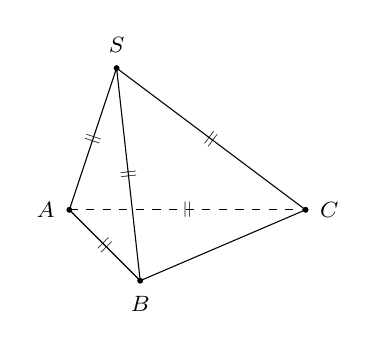
\begin{tikzpicture}[scale=0.6, font=\footnotesize,>=stealth]
	\path
	(0,0) coordinate (A)
	(5,0) coordinate (C)
	(1.5,-1.5) coordinate (B)
	(1,3) coordinate (S)
	;
	\draw (S)--(A)node[midway,sloped,scale=0.7]{$||$}--(B)node[midway,sloped,scale=0.7]{$||$}--(C)--(S)node[midway,sloped,scale=0.7]{$||$} (S)--(B)node[midway,sloped,scale=0.7]{$||$};
	\draw[dashed](A)--(C)node[midway,sloped,scale=0.7]{$||$};
	\foreach \x/\g in {A/180,S/90,C/0,B/-90}\draw[fill=black] (\x) circle (.05) +(\g:.5)node{\footnotesize$\x$};
	\end{tikzpicture}}
	\loigiai{
	\immini{Ta có
	\begin{align*}
	\cos \left(\vec{S C}, \vec{A B}\right) & \ =\dfrac{\vec{S C} \cdot \vec{A B}}{\left|\vec{S C}\right| \cdot\left|\vec{A B}\right|}=\dfrac{\left(\vec{S A}+\vec{A C}\right) \cdot \vec{A B}}{a^2} \\
	 & \ =\dfrac{\vec{S A} \cdot \vec{A B}+\vec{A C} \cdot \vec{A B}}{a^2}.
	\end{align*}
	Từ giả thiết suy ra $S A B$ là tam giác đều và $A B C$ là tam giác vuông cân tại $A$. Từ đó ta tính được
	$\vec{S A} \cdot \vec{A B}=a\cdot a \cdot \cos 120^{\circ}=-\dfrac{a^2}{2}$ và $\vec{A C} \cdot \vec{A B}=0$.\\
	Suy ra $\cos \left(\vec{S C}, \vec{A B}\right)=-\dfrac{1}{2}$.\\
	Vậy $\cos \left(\vec{S C}, \vec{A B}\right)=120^{\circ}$.
	}{
	\begin{tikzpicture}[scale=0.7, font=\footnotesize,>=stealth]
	\path
	(0,0) coordinate (A)
	(5,0) coordinate (C)
	(1.5,-1.5) coordinate (B)
	(1,3) coordinate (S)
	;
	\draw (S)--(A)node[midway,sloped,scale=0.7]{$||$}--(B)node[midway,sloped,scale=0.7]{$||$}--(C)--(S)node[midway,sloped,scale=0.7]{$||$} (S)--(B)node[midway,sloped,scale=0.7]{$||$};
	\draw[dashed](A)--(C)node[midway,sloped,scale=0.7]{$||$};
	\foreach \x/\g in {A/180,S/90,C/0,B/-90}\draw[fill=black] (\x) circle (.05) +(\g:.5)node{\footnotesize$\x$};
	\draw pic[draw,angle radius=0.3cm]{right angle=B--S--C};
	\end{tikzpicture}}
	}
\end{ex} 
%%==========Câu 12
\begin{ex}
	\immini{Cho tứ diện $OABC$ có các cạnh $OA$, $OB$, $OC$ đôi một vuông góc và $OA=OB=OC=1$. Gọi $M$ là trung điểm của cạnh $AB$. Tính góc giữa hai vectơ $\vec{OM}$ và $\vec{AC}$.
	\haicot
	{$90^\circ$}
	{\True $120^\circ$}
	{$60^\circ$}
	{$30^\circ$}}{
	\begin{tikzpicture}[scale=0.4, font=\footnotesize, line join=round, line cap=round]
	\foreach \x\y\t in {0/0/O,3/-3.6/A,7/2/B,0.3/5/C} \coordinate (\t) at (\x,\y);
	\draw (O)--(C)--(B)--(A)--(O);
	\coordinate (M) at ($(A)!1/2!(B)$);
	\draw[-stealth,thick] (A)--(C);
	\draw[-stealth,dashed,thick] (O)--(M);
	\draw[dashed] (O)--(B);
	\foreach \t/\g in {A/-90,B/0,C/90,O/180,M/0} \draw (\t) node[shift={(\g:10pt)}]{$\t$};
	\end{tikzpicture}}
	\loigiai{
	\immini{Đặt $\vec{OA}=\vec{a}$, $\vec{OB}=\vec{b}$, $\vec{OC}=\vec{c}$. \\
	Khi đó, $\left| \vec{a} \right| = \left| \vec{b} \right| = \left| \vec{c} \right| = 1$ và $\vec{a} \cdot \vec{b} = \vec{a} \cdot \vec{c} = \vec{b} \cdot \vec{c} = 0$.\\
	Ta có $\cos \left(\vec{OM},\vec{AC} \right) = \dfrac{\vec{OM} \cdot \vec{AC}}{\left| \vec{OM} \right| \cdot \left| \vec{AC} \right|}$.\\
	Mặt khác do $\vec{OM} = \dfrac{1}{2} \left(\vec{OA}+\vec{OB} \right) = \dfrac{1}{2} \left(\vec{a}+\vec{b} \right)$\\
	và $\vec{AC} = \vec{OC} - \vec{OA} = \vec{c} - \vec{a}$\\
	nên $\begin{aligned}[t]
	\vec{OM} \cdot \vec{AC} & =\dfrac{1}{2} \left(\vec{a}+\vec{b} \right) \cdot \left(\vec{c}-\vec{a} \right) \\
	 & =\dfrac{1}{2} \left(\vec{a} \cdot \vec{c}-\vec{a}^2+ \vec{b} \cdot \vec{c} - \vec{b} \cdot \vec{a} \right) = -\dfrac{1}{2}. \\
	\end{aligned}$
	}
	{\begin{tikzpicture}[scale=0.45, font=\footnotesize, line join=round, line cap=round]
	\foreach \x\y\t in {0/0/O,3/-3.6/A,7/2/B,0.3/5/C} \coordinate (\t) at (\x,\y);
	\draw (O)--(C)--(B)--(A)--(O);
	\coordinate (M) at ($(A)!1/2!(B)$);
	\draw[-stealth,red,very thick] (A)--(C);
	\draw[-stealth,dashed,red,very thick] (O)--(M);
	\draw[dashed] (O)--(B);
	\foreach \t/\g in {A/-90,B/0,C/90,O/180,M/0} \draw (\t) node[shift={(\g:10pt)}]{$\t$};
	\end{tikzpicture}}
	Ta lại có $\left| \vec{OM} \right| = OM =\dfrac{\sqrt{2}}{2}$, $\left| \vec{AC} \right| = AC = \sqrt{2}$. \\
	Do đó $\cos \left(\vec{OM},\vec{AC} \right) = \dfrac{\vec{OM} \cdot \vec{AC}}{\left| \vec{OM} \right| \cdot \left| \vec{AC} \right|} = \dfrac{\dfrac{-1}{2}}{\dfrac{\sqrt{2}}{2} \cdot \sqrt{2}} = \dfrac{-1}{2}$. \\
	Vậy $\left( \vec{OM}, \vec{AC}\right) = 120^\circ$.
	}
\end{ex} 
%%==========Câu 13
\begin{ex}
	Cho hình lập phương $ABCD.A'B'C'D'$ cạnh bằng $a$. Tích vô hướng của hai vectơ $\vec{DD'}$ và $\vec{A'C'}$ bằng
	\choice
	{$\sqrt{2}a^2$}
	{$a^2$}
	{$-\sqrt{2}a^2$}
	{\True $0$}
	\loigiai{
	Ta có: $\vec{A'C'}=\vec{A'D'}+\vec{D'C'}$, mà tứ giác $ADD'A'$ và $DCC'D'$ là hình vuông nên $\vec{DD'} \cdot \vec{A'D'}=\vec{DD'} \cdot \vec{D'C'}=0$. Do đó $\vec{DD'} \cdot \left(\vec{A'D'}+\vec{D'C'}\right)=0$.
	}
\end{ex}
\Closesolutionfile{ans}
\textbf{PHẦN II.} \textit{Câu trắc nghiệm đúng sai. Trong mỗi ý a), b), c), d) ở mỗi câu, học sinh chọn đúng hoặc sai.}\\
\Opensolutionfile{ans}[ans/2H2-B1-d2-2]
%%==========Câu 14
\begin{ex}%[2H2H1-3]
	Trong không gian, cho hai véc-tơ $\vec{a}$ và $\vec{b}$ cùng có độ dài bằng $1$. Biết rằng góc giữa hai véc-tơ đó là $45^{\circ}$.
	\choiceTF
	{\True $\vec{a}\cdot \vec{b}=\dfrac{\sqrt{2}}{2}$}
	{\True $\left( \vec{a}+3 \vec{b}\right) \cdot\left( \vec{a}-2 \vec{b}\right)=-5+\dfrac{\sqrt{2}}{2}$}
	{$\left| \vec{a}+ \vec{b}\right|=2+\sqrt{2} $}
	{$\left| \vec{a}-\sqrt{2}\vec{b}\right|=0$}
	\loigiai{
	\begin{enumerate}[a)]
	\item $\vec{a}\cdot \vec{b}=\left| \vec{a}\right|\cdot \left| \vec{b}\right|\cos \left(\vec{a},\vec{b} \right)=\dfrac{\sqrt{2}}{2}$.
	\item $\left( \vec{a}+3 \vec{b}\right) \cdot\left( \vec{a}-2 \vec{b}\right)=\left| \vec{a}\right|^2+\cdot\vec{a}\cdot \vec{b}-6\left| \vec{b}\right|^2 =1+\cdot\dfrac{\sqrt{2}}{2}-6=-5+\dfrac{\sqrt{2}}{2} $.
	\item $\left( \vec{a}+ \vec{b}\right)^2= \vec{a}^2+2\vec{a}\cdot \vec{b}+\vec{b}^2=1+2\cdot\dfrac{\sqrt{2}}{2}+1=2+\sqrt{2}$. Suy ra $\left| \vec{a}+ \vec{b}\right|=\sqrt{2+\sqrt{2}}$.
	\item $\left( \vec{a}-\sqrt{2} \vec{b}\right)^2= \vec{a}^2+2\sqrt{2}\vec{a}\cdot \vec{b}+2\vec{b}^2=1+2\sqrt{2}\cdot\dfrac{\sqrt{2}}{2}+2=2$. Suy ra $\left| \vec{a}- \sqrt{2}\vec{b}\right|=\sqrt{2}$.
	\end{enumerate}
	}
\end{ex} 
%%==========Câu 15
\begin{ex}%[2H2H1-3]
	\immini{Cho tứ diện đều $ABCD$ có cạnh bằng $a$ và $M$ là trung điểm của $CD$.
	\choiceTF
	{\True $\vec{AM} \cdot \vec{CD}=0$}
	{\True $\vec{AB} \cdot \vec{AC}=\dfrac{a^2}{2}$}
	{\True $\vec{AB}\cdot\vec{CD}=0$}
	{$\vec{AM}\cdot\vec{AB} =-\dfrac{a^2}{2}$}
	}{
	\begin{tikzpicture}[scale=1, font=\footnotesize, line join=round, line cap=round, >=Stealth]
	\def\a{3}
	\path
	(0:0) coordinate (B)
	(5:\a) coordinate (D)
	($(D)+(-135:\a/2)$) coordinate (C)
	($(B)+(65:\a)$) coordinate (A)
	($(C)!.5!(D)$) coordinate (M)
	;
	\draw[->] (A)--(D);
	\draw[->] (A)--(C);
	\draw[->] (A)--(B);
	\draw[->] (A)--(M);
	\draw[dashed] (B)--(D);
	\draw (B)--(C)--(D);
	\foreach \x/\g in {A/90,B/180,C/-90,D/0,M/0}
	\draw[fill=black] 	(\x) circle (.5pt)
	($(\g:.3)+(\x)$) node {$\x$};
	\end{tikzpicture}}
	\loigiai{
	\begin{enumerate}[a)]
	\item Tam giác $ACD$ đều, suy ra $AM$ vuông góc với $CD$ nên $\vec{AM}\cdot \vec{CD}=0$.
	\item Ta có $\begin{aligned}[t]
	 \vec{AB} \cdot \vec{AC} & = |\vec{AB}| \cdot |\vec{AC}| \cdot \cos (\vec{AB},\vec{AC}) \\
	 & = AB \cdot AC \cdot \cos \widehat{BAC} \\
	 & = a \cdot a \cdot \cos {60^0} \\
	 & = \dfrac{a^2}{2}.
	 \end{aligned}$\\
	\item Ta có $\vec{AB} \cdot \vec{CD}=(\vec{AM}+\vec{MB}) \cdot \vec{CD}=\vec{AM} \cdot \vec{CD} +\vec{MB} \cdot \vec{CD}$.\\
	 Mà $AM$, $BM$ là trung tuyến của các tam giác đều $ACD$, $BCD$ nên $\vec{AM} \perp \vec{CD}, \vec{MB} \perp \vec{CD}$.\\
	 Suy ra $\vec{AM} \cdot \vec{CD} = \vec{MB} \cdot \vec{CD} = 0$.\\
	 Từ các kết quả trên ta có $\vec{AM} \cdot \vec{CD}=0$.
	 Suy ra $(\vec{AB}, \vec{CD})=90^\circ$.
	\item Ta có $\vec{AM} = \dfrac{1}{2}(\vec{AC} + \vec{AD})$, suy ra
	 \[ \vec{AB} \cdot \vec{AM} = \vec{AB} \cdot \frac{1}{2}(\vec{AC} +\vec{AD}) = \frac{1}{2}(\vec{AB} \cdot \vec{AC} + \vec{AB} \cdot \vec{AD}) = \frac{1}{2}\left(\frac{a^2}{2} + \frac{a^2}{2}\right) = \dfrac{a^2}{2}.\]
	\end{enumerate}
	}
\end{ex} 
%%==========Câu 16
\begin{ex}
	\immini{
	Một chất điểm ở vị trí đỉnh $A$ của hình lập phương $ABCD.A'B'C'D'$. Chất điểm chịu tác động bởi ba lực $\vec{a}$, $\vec{b}$, $\vec{c}$ lần lượt cùng hướng với $\vec{AD}$, $\vec{AB}$ và $\vec{AC'}$ như hình vẽ. Độ lớn của các lực $\vec{a}$, $\vec{b}$ và $\vec{c}$ tương ứng là $10$ N, $10$ N và $20$ N.
	\choiceTF
	{$\vec{a}+\vec{b}=\vec{c}$}
	{$\big|\vec{a}+\vec{b}\big|=20$ (N)}
	{\True $\big|\vec{a}+\vec{c}\big|=\big|\vec{b}+\vec{c}\big|$}
	{\True $\big|\vec{a}+\vec{b}+\vec{c}\big|=32{,}59$ (N) (\textit{làm tròn kết quả đến hàng phần mười})}
	}{\hspace{0.5cm}
	\begin{tikzpicture}[line join=round, line cap = round, >=stealth, scale=0.65,font=\footnotesize]
	\path
	(0,0) coordinate (A')
	(-1.5,-1.5) coordinate (D')
	(2,-1.5) coordinate (C')
	(3.5,0) coordinate (B')
	(0,3.5) coordinate (A)
	($(A)+(B')-(A')$) coordinate (B)
	($(A)+(C')-(A')$) coordinate (C)
	($(A)+(D')-(A')$) coordinate (D)
	($(A)!1/2!(D)$) coordinate (M)
	($(A)!1/2!(B)$) coordinate (N)
	($(A)!1/2!(C')$) coordinate (P)
	;
	\draw[->,thick](A)--node [left]{$\vec{a}$}(M);
	\draw[->,thick](A)--node [above]{$\vec{b}$}(N);
	\draw[->,thick](A)--node[right]{$\vec{c}$}(P);
	\draw[dashed] (D')--(A')--(B') (A')--(A)--(C');
	\draw (D)--(C)--(B)--(A)--(D)--(D')--(C')--(C) (C')--(B')--(B);
	\draw pic[draw,angle eccentricity=1.2,angle radius=0.25cm]{right angle= D--A--B};
	\foreach \x/\g in {A/90,B/80,C/-40,D/110,A'/160,B'/-65,C'/-90,D'/-100} \fill[black](\x) circle (1pt) ($(\x)+(\g:3mm)$)node{$\x$};
	\end{tikzpicture}
	}
	\loigiai{
	Từ giả thiết, ta có $\vec{a} \perp \vec{b};\cos\left(\vec{a},\vec{c}\right)= \cos \widehat{DAC'}= \dfrac{1}{\sqrt3}; \cos \left(\vec{b},\vec{c}\right)= \cos \widehat{BAC'}= \dfrac{1}{\sqrt3}$.\\
	\begin{enumerate}[a)]
	\item Giả sử $\vec{a}+\vec{b}=\vec{d}$. Theo quy tắc hình bình hành thì $\vec{d}$ cùng hướng với $\vec{AC}$. Suy ra $\vec{a}+\vec{b}\ne \vec{c}$
	\item $\big|\vec{a}+\vec{b}\big|=10\sqrt{2}$ (đường chéo hình vuông cạnh bằng 10).
	\item Ta có
	 \begin{itemize}
	 \item [$\bullet$] $\big(\vec{a}+\vec{c}\big)^2=|\vec{a}|^2+2\vec{a} \cdot \vec{c}+|\vec{c}|^2=10^2+2.10.20.\dfrac{1}{\sqrt{3}}+20^2=500+\dfrac{400\sqrt{3}}{3}$.\\
	 Suy ra $\big|\vec{a}+\vec{c}\big|=\sqrt{500+\dfrac{400\sqrt{3}}{3}}$.
	 \item [$\bullet$] $\big(\vec{b}+\vec{c}\big)^2=|\vec{b}|^2+2\vec{b} \cdot \vec{c}+|\vec{c}|^2=10^2+2.10.20.\dfrac{1}{\sqrt{3}}+20^2=500+\dfrac{400\sqrt{3}}{3}$.\\
	 Suy ra $\big|\vec{b}+\vec{c}\big|=\sqrt{500+\dfrac{400\sqrt{3}}{3}}$.
	 \end{itemize}
	 Vậy $\big|\vec{a}+\vec{c}\big|=\big|\vec{b}+\vec{c}\big|$.
	\item Giả sử lực tổng hợp là $\vec{m}$, tức là $\vec{m}=\vec{a}+\vec{b}+\vec{c}$.\\
	 Do đó
	 \allowdisplaybreaks
	 \begin{eqnarray*}
	 \vec{m}=\vec{a}+\vec{b}+\vec{c} &\Leftrightarrow& \left|\vec{m}\right|^2= \left(\vec{a}+\vec{b}+\vec{c}\right)^2\\
	 &\Leftrightarrow& \left|\vec{m}\right|^2= \vec{a}^2+\vec{b}^2+\vec{c}^2+2\vec{a}\cdot\vec{b}+2\vec{b}\cdot\vec{c}+2\vec{c}\cdot\vec{a}\\
	 &\Leftrightarrow& \left|\vec{m}\right|^2= 10^2+10^2+20^2+0+2\cdot 10\cdot 20 \cdot \dfrac{1}{\sqrt3} +2\cdot 10\cdot 20 \cdot \dfrac{1}{\sqrt3}\\
	 &\Leftrightarrow& \left|\vec{m}\right|^2= 10^2+10^2+20^2+0+2\cdot 10\cdot 20 \cdot \dfrac{1}{\sqrt3} +2\cdot 10\cdot 20 \cdot \dfrac{1}{\sqrt3}\\
	 &\Leftrightarrow& \left|\vec{m}\right| \approx 32{,}59.
	 \end{eqnarray*}
	 Vậy cường độ hợp lực của $\vec{a}$, $\vec{b}$ và $\vec{c}$ là $\approx 32{,}59$ (N).
	\end{enumerate}
	}
\end{ex} 
%%==========Câu 17
\begin{ex}
	Cho hình chóp $S.ABCD$ có đáy $ABCD$ là hình chữ nhật. Biết rằng cạnh $AB=a$, $AD=2a$, cạnh bên $SA=2a$ và vuông góc với mặt đáy. Gọi $M$, $N$ lần lượt là trung điểm của các cạnh $SB$, $SD$. Các mệnh đề sau đúng hay sai ?
	\choiceTF
	{Hai vectơ $\vec{AB}$, $\vec{CD}$ là hai vectơ cùng phương, cùng hướng}
	{Góc giữa hai vectơ $\vec{SC}$ và $\vec{AC}$ bằng $60^\circ $}
	{\True Tích vô hướng $\vec{AM} \cdot \vec{AB}=\dfrac{a^2}{2}$}
	{Độ dài của vectơ $\vec{AM}-\vec{AN}$ là $\dfrac{a\sqrt{3}}{2}$}
	\loigiai{
	\begin{center}
	\begin{tikzpicture}[line join = round, line cap = round, thick, font = \small, scale = .7]
	\path
	(0:0) coordinate (A)
	+(0:5) coordinate (B)
	+(-150:2.5) coordinate (D)
	+(90:5) coordinate (S)
	($(B)+(D)-(A)$) coordinate (C)
	($(S)!.5!(B)$) coordinate (M)
	($(S)!.5!(D)$) coordinate (N)
	;
	\draw[dashed]
	(D)--(A)--(B) (C)--(A)--(S) (M)--(A)--(N)
	;
	\draw
	(D)--(C)--(B)
	(S)--(B) (S)--(C) (S)--(D)
	\foreach \x/\y/\z in {S/A/B,S/A/D}{
	pic[draw, angle radius = 6pt]{right angle = \x--\y--\z}
	}
	;
	\foreach \x/\g in {A/135,B/0,C/-45,D/-135,S/90,M/45,N/135}
	\fill (\x) circle (1.5pt)
	+(\g:3.5mm) node {$\x$};
	\end{tikzpicture}
	\end{center}
	\begin{enumerate}[a)]
	\item $\vec{AB}=-\vec{CD}$. Suy ra hai vectơ $\vec{AB}$, $\vec{CD}$ là hai vectơ ngược hướng.
	\item Ta có: $ABCD$ là hình chữ nhật nên: $AC=\sqrt{AB^2+AD^2}=a\sqrt{5}$.\\
	 Hình chóp $S.ABCD$ có $SA$ vuông góc với mặt đáy nên tam giác $SAC$ là tam giác vuông tại $A$. Suy ra: $\tan \widehat{SCA}=\dfrac{SA}{AC}=\dfrac{2a}{a\sqrt{5}}\Rightarrow \widehat{SCA}\approx 41^\circ 48'$.\\
	 Ta có: $\left(\vec{SC},\vec{AC}\right)=\left(\vec{CS},\vec{CA}\right)=\widehat{SCA}\approx 41^\circ 48'$.
	\item Hình chóp $S.ABCD$ có $SA$ vuông góc với mặt đáy nên tam giác $SAB$ là tam giác vuông tại $A$.\\
	 Suy ra: $SB=\sqrt{SA^2+AB^2}=a\sqrt{5}$.\\
	 Trong tam giác $SAB$ vuông tại $A$ có $AM$ là đường trung tuyến nên: \\
	 $AM=\dfrac{1}{2}SB=\dfrac{a\sqrt{5}}{2}$.\\
	 Lại có: $M$ là trung điểm của $SB$ nên $MB=\dfrac{1}{2}SB=\dfrac{a\sqrt{5}}{2}$. \\
	 Ta tính được: $\cos \widehat{MAB}=\dfrac{MA^2+AB^2-MB^2}{2MA \cdot AB}=\dfrac{\sqrt{5}}{5}$.\\
	 Mà: $\left(\vec{AM},\vec{AB}\right)=\widehat{MAB}$, suy ra: \\
	 $\vec{AM}\cdot \vec{AB}=\left| \vec{AM} \right| \cdot \left| \vec{AB} \right| \cdot \cos \left(\vec{AM},\vec{AB}\right)=\dfrac{a\sqrt{5}}{2} \cdot a \cdot \dfrac{\sqrt{5}}{5}=\dfrac{a^2}{2}$.
	\item Ta có: $M$, $N$ lần lượt là trung điểm của các cạnh $SB$, $SD$ nên $MN$ là đường trung bình của tam giác $SBD$.
	 Do đó: $MN=\dfrac{1}{2}BD=\sqrt{AB^2+AD^2}=\dfrac{a\sqrt{5}}{2}$.\\
	 Suy ra: $\left| \vec{AM}-\vec{AN} \right| =\left| \vec{MN} \right| =\dfrac{a\sqrt{5}}{2}$.
	\end{enumerate}
	}
\end{ex}
%%==========Câu 18
\begin{ex}
	Cho hình lập phương $ABCD.A'B'C'D'$ có cạnh bằng $a$. Trên các cạnh $AA'$, $CC'$ lần lượt lấy các điểm $M$, $N$ sao cho $AM=\dfrac{2}{3}AA'$, $CN=NC'$. Các mệnh đề sau đúng hay sai?
	\choiceTF
	{Góc giữa hai vectơ $\vec{AN}$ và $\vec{AC}$ bằng $60^\circ $}
	{\True Độ dài của vectơ $\vec{MN}+\vec{AM}$ là $\dfrac{3a}{2}$}
	{Tích vô hướng $\vec{AN}\cdot \vec{AC}=a^2$}
	{\True Tích vô hướng $\vec{MN}\cdot \vec{A'C'}=2a^2$}
	\loigiai{
	\begin{center}
	\begin{tikzpicture}[line join = round, line cap = round, thick, font = \small, scale = .7]
	\def \canh{4}
	\path
	(0:0) coordinate (D')
	+(90:\canh) coordinate (D)
	+(0:\canh) coordinate (C')
	+(40:.4*\canh) coordinate (A')
	($(C')+(D)-(D')$) coordinate (C)
	($(D)+(A')-(D')$) coordinate (A)
	($(C')+(A')-(D')$) coordinate (B')
	($(C)+(A)-(D)$) coordinate (B)
	($(A)!2/3!(A')$) coordinate (M)
	($(C)!.5!(C')$) coordinate (N)
	($(C)!2/3!(C')$) coordinate (M')
	;
	\draw[dashed]
	(A')--(A) (A')--(B') (A')--(D') (M')--(M)--(N)
	;
	\draw
	(A)--(B)--(B')--(C')--(D')--(D)--cycle
	(C)--(B) (C)--(D) (C)--(C')
	;
	\foreach \x/\g in {D'/-90,C'/-90,D/180,A'/135,C/-45,A/90,B'/0,B/90,M/180,N/0,M'/0}
	\fill (\x) circle (1.5pt)
	+(\g:3mm) node {$\x$};
	\end{tikzpicture}
	\end{center}
	\begin{enumerate}[a)]
	\item Ta có: $AC=\sqrt{AB^2+AC^2}=a\sqrt{2}$.\\
	 Lại có: $CN=NC'$ nên $CN=NC'=\dfrac{a}{2}$.\\
	 $ABCD.A'B'C'D'$ là hình lập phương nên tam giác $NAC$ là tam giác vuông tại $C$.\\
	 Suy ra: $\tan NAC=\dfrac{CN}{AC}=\dfrac{\sqrt{2}}{4}\Rightarrow \widehat{NAC}\approx 19^\circ 28'$\\
	 Ta có: $\left(\vec{AN},\vec{AC}\right)=\widehat{NAC}\approx 19^\circ 28'$.
	\item Trong tam giác $NAC$ vuông tại $C$ có: $AN=\sqrt{AC^2+CN^2}=\dfrac{3a}{2}$.\\
	 Ta có: $\left| \vec{MN}+\vec{AM} \right| =\left| \vec{AN} \right| =\dfrac{3a}{2}$.
	\item Ta có: $\tan \widehat{NAC}=\dfrac{\sqrt{2}}{4}\Rightarrow \cos \widehat{NAC}=\dfrac{2\sqrt{2}}{3}$ (Do $\widehat{NAC}<90^\circ $).\\
	 Do đó: $\vec{AN}\cdot \vec{AC}=\left| \vec{AN} \right| \cdot \left| \vec{AC} \right| \cdot \cos \left(\vec{AN},\vec{AC}\right)=\dfrac{3a}{2} \cdot a\sqrt{2} \cdot \dfrac{2\sqrt{2}}{3}=2a^2$.
	\item Trên cạnh $CC'$ lấy điểm $M'$ sao cho: $\dfrac{CM'}{CC'}=\dfrac{2}{3}$.\\
	 Suy ra: $\heva{& NM'=NC'-M'C'=\dfrac{a}{6} \\ & MM'\parallel AC \\ & MM'=AC=a\sqrt{2}} $.\\
	 Ta có: $\cos \widehat{NMM'}=\dfrac{NM^2+M'M^2-M'N^2}{2 \cdot NM \cdot M'M}=\dfrac{6\sqrt{146}}{73}$.\\
	 Mặt khác: $\left(\vec{MN},\vec{A'C'}\right)=\left(\vec{MN},\vec{MM'}\right)=\widehat{NMM'}$.\\
	 Tam giác $MNM'$ vuông tại $M'$ có: $MN=\sqrt{M'N^2+M'M^2}=\dfrac{a\sqrt{73}}{6}$.\\
	 Do đó: $\vec{MN}\cdot \vec{A'C'}=\left| \vec{MN} \right| \cdot \left| \vec{A'C'} \right| \cdot \cos \left(\vec{MN},\vec{A'C'}\right)=2a^2$.
	\end{enumerate}
	}
\end{ex}
%%==========Câu 19
\begin{ex}
	Cho hình lăng trụ đứng $ABC.A'B'C'$ đáy là tam giác đều cạnh $2a,AA'=a\sqrt{3}$. $H$, $K$ lần lượt là trung điểm $BC$, $B'C'$. Các mệnh đề sau đúng hay sai?
	\choiceTF
	{Hai vectơ $\vec{AH}$, $\vec{KA'}$ là hai vectơ cùng phương, cùng hướng}
	{Góc giữa hai vectơ $\vec{A'H}$ và $\vec{AH}$ bằng $60^\circ $}
	{Tích vô hướng $\vec{AK}\cdot \vec{AB'}=\dfrac{5a^2}{2}$}
	{\True Độ dài của vectơ $\vec{AK}+\vec{AH}$ là $\dfrac{a\sqrt{3}}{2}$}
	\loigiai{
	\begin{center}
	\begin{tikzpicture}[line join = round, line cap = round, thick, font = \small, scale = .7]
	\path
	(0:0) coordinate (A)
	+(0:4) coordinate (C)
	+(-50:2) coordinate (B)
	+(90:4) coordinate (A')
	($(A')+(B)-(A)$) coordinate (B')
	($(A')+(C)-(A)$) coordinate (C')
	($(B)!.5!(C)$) coordinate (H)
	($(B')!.5!(C')$) coordinate (K)
	($(H)!.5!(K)$) coordinate (I)
	;
	\draw[dashed]
	(A)--(C) (H)--(A)--(K) (A)--(I)
	;
	\draw
	(A)--(B)--(C)--(C')--(A')--cycle
	(B')--(A') (B')--(B) (B')--(C') (A')--(K)--(H)
	;
	\foreach \x/\g in {A/180,B/-90,C/0,A'/-180,B'/-150,C'/0,H/-45,K/-30,I/0}
	\fill (\x) circle (1.5pt)
	+(\g:3mm) node {$\x$};
	\end{tikzpicture}
	\end{center}
	\begin{enumerate}[a)]
	\item Ta có tam giác $\triangle ABC,\triangle A'B'C'$ đều cạnh $2a$ suy ra $A'K=AH=a\sqrt{3}$\\
	 Xét tứ giác $AA'KH$ có $AA'=KH=AH=A'K=a\sqrt{3}$, $AA'\perp AH$ suy ra tứ giác $AA'KH$ là hình vuông , từ đó dễ thấy hai vectơ $\vec{AH}$, $\vec{KA'}$ là hai vecto cùng phương ngược hướng.
	\item Ta có: $AA'KH$ là hình vuông suy ra $\widehat{A'HA}=45^\circ $\\
	 Có $A'A\perp AH\Rightarrow \triangle A'AH$ vuông tại $A\Rightarrow \left(\vec{A'H},\vec{AH}\right)=\widehat{A'HA}=45^\circ $.
	\item Ta có $\triangle AB'C'$ cân tại $A$, suy ra $AK\perp B'C'$, $AK=a\sqrt{6},B'K=a$\\
	 $AB'=\sqrt{AB^2+BB'^2}=\sqrt{4a^2+3a^2}=a\sqrt{7}$\\
	 Xét $\triangle AKB'$ có $\cos \widehat{KAB'}=\dfrac{AK}{AB'}=\dfrac{a\sqrt{6}}{a\sqrt{7}}=\sqrt{\dfrac{6}{7}}$.\\
	 $\vec{AK} \cdot \vec{AB'}=AK \cdot AB'\cdot \cos \widehat{KAB'}=a\sqrt{6} \cdot a\sqrt{7} \cdot \sqrt{\dfrac{6}{7}}=6a^2$.
	\item Gọi $I$ là trung điểm $HK\Rightarrow IH=\dfrac{a\sqrt{3}}{2}$, $AI=\sqrt{IH^2+AH^2}=\sqrt{\dfrac{3a^2}{4}+3a^2}=\dfrac{a\sqrt{15}}{2}$.\\
	 Ta có $\left| \vec{AK}+\vec{AH} \right| =\left| 2 \cdot \vec{AI} \right| =2AI=a\sqrt{15}$.
	\end{enumerate}
	}
\end{ex}
%%==========Câu 20
\begin{ex}
	Cho tứ diện đều $ABCD$ cạnh $a$. $E$ là điểm trên đoạn $CD$ sao cho $ED=2CE$. Các mệnh đề sau đúng hay sai?
	\choiceTF
	{Có $6$ vectơ (khác vectơ $\vec{0}$) có điểm đầu và điểm cuối được tạo thành từ các đỉnh của tứ diện}
	{Góc giữa hai vectơ $\vec{AB}$ và $\vec{BC}$ bằng $60^\circ $}
	{Nếu $\vec{BE}=m\vec{BA}+n\vec{BC}+p\vec{BD}$ thì $m+n+p=\dfrac{2}{3}$}
	{\True Tích vô hướng $\vec{AD} \cdot \vec{BE}=\dfrac{a^2}{6}$}
	\loigiai{
	\begin{center}
	\begin{tikzpicture}[line join = round, line cap = round, thick, font = \small, scale = .7]
	\path
	(0:0) coordinate (B)
	+(0:5) coordinate (C)
	+(-70:2) coordinate (D)
	+(70:4) coordinate (A)
	($(C)!1/3!(D)$) coordinate (E)
	;
	\draw[dashed]
	(B)--(C) (B)--(E)
	;
	\draw
	(A)--(B)--(D)--(C)--cycle
	(E)--(A)--(D)
	;
	\foreach \x/\g in {B/180,C/0,D/-90,A/90,E/-45}
	\fill (\x) circle (1.5pt)
	+(\g:3mm) node {$\x$};
	\end{tikzpicture}
	\end{center}
	\begin{enumerate}[a)]
	\item Số vectơ (khác $\vec{0}$) có điểm đầu và điểm cuối được tạo thành từ các đỉnh của tứ diện là $A_4^2=12$.
	\item $(\vec{AB},\vec{BC})=180^\circ-(\vec{BA},\vec{BC})={{180}^\circ}-\widehat{ABC}=120^\circ$.
	\item $\vec{BE}=\vec{BC}+\vec{CE}=\vec{BC}+\dfrac{1}{3}\vec{CD}=\vec{BC}+\dfrac{1}{3}\left(\vec{BD}-\vec{BC}\right)=\dfrac{2}{3}\vec{BC}+\dfrac{1}{3}\vec{BD}$.\\
	 Do đó $m=0$,$n=\dfrac{2}{3}$,$p=\dfrac{1}{3}$. Suy ra $m+n+p=1$.
	\item Ta có: $\vec{BE}=\vec{AE}-\vec{AB}=\left(\vec{AC}+\vec{CE}\right)-\vec{AB}=\vec{AC}+\dfrac{1}{3}\vec{CD}-\vec{AB}$\\
	 $=\vec{AC}+\dfrac{1}{3}\left(\vec{AD}-\vec{AC}\right)-\vec{AB}=\dfrac{2}{3}\vec{AC}+\dfrac{1}{3}\vec{AD}-\vec{AB}$\\
	 Suy ra: $\vec{AD} \cdot \vec{BE}=\vec{AD} \cdot \left(\dfrac{2}{3}\vec{AC}+\dfrac{1}{3}\vec{AD}-\vec{AB}\right)=\dfrac{2}{3} \cdot \vec{AD} \cdot \vec{AC}+\dfrac{1}{3} \cdot {{\vec{AD}}^2}-\vec{AD} \cdot \vec{AB}$\\
	 $=\dfrac{2}{3} \cdot a \cdot a \cdot \cos 60^\circ +\dfrac{1}{3}a^2-a \cdot a \cdot \cos 60^\circ =\dfrac{a^2}{6}$.
	\end{enumerate}
	}
\end{ex}
%%==========Câu 21
\begin{ex}
	Cho tứ diện $ABCD$ có cạnh $a$. Gọi $M$, $N$ lần lượt là trung điểm của $AB$, $CD$. Các mệnh đề sau đúng hay sai?
	\choiceTF
	{$\vec{AB}$ và $\vec{CD}$ cùng hướng}
	{\True $\vec{EA}+\vec{EB}+\vec{EC}+\vec{ED}=\vec{0}$ với $E$ là trung điểm $MN$}
	{\True $\vec{AB} \cdot \vec{CD}+\vec{AC} \cdot \vec{DB}+\vec{AD} \cdot \vec{BC}=\vec{0}$}
	{\True Điểm $I$ xác định bởi $P=3\vec{IA}^2+\vec{IB}^2+\vec{IC}^2+\vec{ID}^2$ có giá trị nhỏ nhất. Khi đó giá trị nhỏ nhất của $P$ là $2a^2$}
	\loigiai{
	\begin{center}
	\begin{tikzpicture}[line join = round, line cap = round, thick, font = \small, scale = 1]
	\path 
	(0:0) coordinate (B)
	+(0:5) coordinate (C)
	+(-45:2) coordinate (D)
	+(70:4) coordinate (A)
	($(A)!.5!(B)$) coordinate (M)
	($(C)!.5!(D)$) coordinate (N)
	($(M)!.5!(N)$) coordinate (E)
	($(B)!2/3!(N)$) coordinate (G)
	($(A)!.5!(G)$) coordinate (O)
	;
	\draw[dashed] 
	(B)--(C) (A)--(G) (M)--(N)
	;
	\draw 
	(A)--(B)--(D)--(C)--cycle
	(A)--(D)
	;
	\foreach \x/\g in {B/180,C/0,D/-90,G/0,A/90,M/135,N/-45,E/0,O/0}
	\fill (\x) circle (1.5pt)
	+(\g:3mm) node {$\x$};
	\end{tikzpicture}
	\end{center}
	\begin{enumerate}[a)]
	\item $\vec{AB}$ và $\vec{CD}$ ngược hướng.
	\item Vì $M$ là trung điểm $AB$ nên $\vec{EA}+\vec{EB}=2\vec{EM}$, $N$ là trung điểm $CD$ nên $\vec{EC}+\vec{ED}=2\vec{EN}$.\\
	Ta có $\vec{EA}+\vec{EB}+\vec{EC}+\vec{ED}=2\left(\vec{EM}+\vec{EN}\right)=\vec{0}$.
	\item $\begin{aligned}[t]
	&\vec{AB} \cdot \vec{CD}+\vec{AC} \cdot \vec{DB}+\vec{AD} \cdot \vec{BC}=\left(\vec{AC}+\vec{CB}\right) \cdot \vec{CD}+\vec{AC} \cdot \vec{DB}+\vec{AD} \cdot \vec{BC}\\
	 = & \vec{AC} \cdot \left(\vec{CD}+\vec{DB}\right)+\vec{AD} \cdot \vec{BC}+\vec{CB \cdot }\vec{CD}=\vec{AC} \cdot \vec{CB}+\vec{AD} \cdot \vec{BC}+\vec{CB \cdot }\vec{CD} \\
	 = &\vec{CB}\left(\vec{AC}-\vec{AD}\right)+\vec{CB \cdot }\vec{CD}=\vec{0} 
	\end{aligned}$
	\item Gọi $O$ là điểm thoả mãn hệ thức $3\vec{OA}+\vec{OB}+\vec{OC}+\vec{OD}=\vec{0}$ suy ra $O$ cố định vì $A$, $B,C$, $D$ cố định. Ta có
	\begin{align*}
	P& =3\vec{IA}^2+\vec{IB}^2+\vec{IC}^2+\vec{ID}^2 \\
	& =3\left(\vec{IO}+\vec{OA}\right)^2+\left(\vec{IO}+\vec{OB}\right)^2+\left(\vec{IO}+\vec{OC}\right)^2+\left(\vec{IO}+\vec{OD}\right)^2 \\
	& =6IO^2+3OA^2+OB^2+OC^2+OD^2+2\vec{IO}\left(3\vec{OA}+\vec{OB}+\vec{OC}+\vec{OD}\right) \\
	& =6IO^2+3OA^2+OB^2+OC^2+OD^2.
	\end{align*}
	Do đó để $P$ nhỏ nhất thì $I$ trùng với $O$. Gọi $G$ là trọng tâm tam giác $BCD$.\\
	Vì $3\vec{OA}+\vec{OB}+\vec{OC}+\vec{OD}=3\vec{OA}+\left(\vec{OB}+\vec{OC}+\vec{OD}\right) =3\vec{OA}+3\vec{OG}$ nên $\vec{OA}+\vec{OG}=\vec{0}$.\\	
	Suy ra $O$ là trung điểm của $AG$.\\
	Ta có $BG=\dfrac{2}{3} \cdot \dfrac{a\sqrt{3}}{2}=\dfrac{a}{\sqrt{3}}\Rightarrow AG=\sqrt{AB^2-BG^2}=\sqrt{a^2-{{\left(\dfrac{a}{\sqrt{3}}\right)}^2}}=\dfrac{a\sqrt{2}}{\sqrt{3}}$\\
	$\Rightarrow OA=\dfrac{1}{2}AG=\dfrac{a}{\sqrt{6}}\Rightarrow OA^2=\dfrac{a^2}{6}$.\\
	Lại có $OD^2=OC^2=OB^2=OG^2+BG^2=\dfrac{a^2}{6}+\dfrac{a^2}{3}=\dfrac{a^2}{2}$.\\
	Vậy giá trị nhỏ nhất là $P=3 \cdot \dfrac{a^2}{6}+3 \cdot \dfrac{a^2}{2}=2a^2$ khi $I$ trùng với $O$.
	\end{enumerate}
	}
\end{ex}
\textbf{PHẦN III.} \textit{Câu trắc nghiệm trả lời ngắn.}\\
%%==========Câu 22
\begin{ex}
	Cho tứ diện đều $ABCD$ có cạnh bằng $4$. Giá trị tích vô hướng $\vec{AB}\left(\vec{AB}-\vec{CA}\right)$ bằng
	\loigiai{
	\SA{24}
	$\begin{aligned}[t]
	\vec{AB}\left(\vec{AB}-\vec{CA}\right)
	 & =\vec{AB} \cdot \vec{AB}+\vec{AB} \cdot \vec{AC}={{\vec{AB}}^2}+| \vec{AB}| \cdot | \vec{AC}| \cdot \cos \left(\vec{AB},\vec{AC}\right) \\
	 & =AB^2+AB \cdot AC \cdot \cos \left(\widehat{BAC}\right)=4^2+4 \cdot 4 \cdot \cos 60^\circ=4^2+\dfrac{4^2}{2}=\dfrac{{{3 \cdot 4}^2}}{2}=24.
	\end{aligned}$
	}
\end{ex}
%%==========Câu 23
\begin{ex}
	Trong không gian, cho hai vectơ $\vec{a}$ và $\vec{b}$ có cùng độ dài bằng $6$. Biết độ dài của vectơ $\vec{a}+2\vec{b}$ bằng $6\sqrt{3}$. Biết số đo góc giữa hai vectơ $\vec{a}$ và $\vec{b}$ là $x$ độ. Giá trị của $x$ là bao nhiêu?
	\loigiai{
	\SA{120}
	$\vec{a} \cdot \vec{b} = \dfrac{1}{4} \left[\left(\vec{a}+2 \vec{b}\right)^2 - \vec{a}^2 - 4\vec{b}^2\right]
	= \dfrac{1}{4} \left[\left|\vec{a}+2 \vec{b}\right|^2 - |\vec{a}|^2 - 4|\vec{b}|^2\right]
	= \dfrac{1}{4} \left[\left(6\sqrt{3}\right)^2 - 6^2 - 4\cdot 6^2\right] = -18$.\\
	Lại có $\vec{a} \cdot \vec{b}=| \vec{a}| \cdot | \vec{b}| \cdot \cos \left(\vec{a}\,,\vec{b}\right)\Leftrightarrow \cos \left(\vec{a}\,,\vec{b}\right)=\dfrac{\vec{a} \cdot \vec{b}}{| \vec{a}| \cdot | \vec{b}|}=\dfrac{-18}{6 \cdot 6}=\dfrac{-1}{2}\Leftrightarrow \left(\vec{a}\,,\vec{b}\right)=120^\circ $.\\
	Khi đó góc giữa hai vectơ $\vec{a}$ và $\vec{b}$ là $120^\circ $.
	}
\end{ex}
%%==========Câu 24
\begin{ex}
	Cho hình lập phương $ABCD.A'B'C'D'$ có cạnh bằng $2$. Tính $\vec{AB} \cdot \vec{A'C'}$.
	\loigiai{
	\SA{4}
	Ta có: $\left(\vec{AB},\vec{A'C'}\right)=\left(\vec{AB},\vec{AC}\right)=45^\circ $.\\
	Khi đó: $\vec{AB} \cdot \vec{A'C'}=AB \cdot A'C'\cdot \cos \left(\vec{AB},\vec{A'C'}\right)=2 \cdot 2\sqrt{2} \cdot \cos 45^\circ =4$.
	}
\end{ex}
%%==========Câu 25
\begin{ex}
	Cho tứ diện $ABCD$, gọi $M$, $N$ lần lượt là trung điểm của $BC$ và $AD$, biết $AB=a$, $CD=a$, $MN=\dfrac{a\sqrt{3}}{2}$. Tìm số đo (đơn vị độ) góc giữa hai đường thẳng $AB$ và $CD$.
	\loigiai{
	\SA{60}
	\begin{center}
	\begin{tikzpicture}[line join = round, line cap = round, thick, font = \small, scale = .7]
	\path
	(0:0) coordinate (B)
	+(0:5) coordinate (D)
	+(-30:4) coordinate (C)
	+(70:4) coordinate (A)
	($(B)!1/2!(C)$) coordinate (M)
	($(A)!1/2!(D)$) coordinate (N)
	($(A)!1/2!(C)$) coordinate (I)
	;
	\draw[dashed]
	(B)--(D) (M)--(N)
	;
	\draw
	(A)--(B)--(C)--(D)--cycle
	(A)--(C) (M)--(I)--(N)
	;
	\foreach \x/\g in {B/180,D/0,C/-90,A/90,M/-135,I/180,N/45}
	\fill (\x) circle (1.5pt)
	+(\g:3mm) node {$\x$};
	\end{tikzpicture}
	\end{center}
	Gọi $I$ là trung điểm của $AC$.\\
	Ta có $\heva{& IM \parallel AB \\& IN \parallel CD}\Rightarrow \widehat{\left(AB,CD\right)}=\widehat{\left(IM,IN\right)}$.\\
	Đặt $\widehat{MIN}=\alpha $. Xét tam giác $IMN$, có: $IM=\dfrac{AB}{2}=\dfrac{a}{2}$, $IN=\dfrac{CD}{2}=\dfrac{a}{2}$, $MN=\dfrac{a\sqrt{3}}{2}$.\\
	Theo định lý cosin, có $\cos \alpha =\dfrac{IM^2+IN^2-MN^2}{2 \cdot IM \cdot IN}=-\dfrac{1}{2}<0$.\\
	$\Rightarrow \widehat{MIN}=120^\circ \Rightarrow \widehat{\left(AB,CD\right)}=60^\circ $.
	}
\end{ex}
%%==========Câu 26
\begin{ex}
	Cho hình lập phương $ABCD.A'B'C'D'$. Góc giữa hai vectơ $\vec{A'B}$ và $\vec{AC'}$ bằng
	\loigiai{
	\SA{90}
	$\vec{A'B}=\vec{A'A}+\vec{AB}=\vec{AB}-\vec{AA'}$.\\
	$\vec{AC'}=\vec{AB}+\vec{AD}+\vec{AA'}$.\\
	$\Rightarrow \vec{A'B} \cdot \vec{AC'} = \left(\vec{AB}-\vec{AA'}\right) \cdot \left(\vec{AB}+\vec{AD}+\vec{AA'}\right)={{\vec{AB}}^2}-{{\vec{AA'}}^2}=0$.\\
	$\Rightarrow$ Góc giữa hai vectơ $\vec{A'B}$ và $\vec{AC'}$ bằng $90^\circ$.
	}
\end{ex}
%%==========Câu 27
\begin{ex}
	Cho hình chóp $S.ABC$ có $SA$, $SB$, $SC$ đôi một vuông góc nhau và $SA=SB=SC=a$. Gọi $M$ là trung điểm của $AB$. Góc giữa hai vectơ $\vec{SM}$ và $\vec{BC}$ bằng
	\loigiai{
	\shortans{120}	
	Ta có $\cos \left(\vec{SM},\vec{BC}\right)=\dfrac{\vec{SM} \cdot \vec{BC}}{|\vec{SM}| \cdot |\vec{BC}|}=\dfrac{\vec{SM} \cdot \vec{BC}}{SM \cdot BC}$.\\
	\begin{align*}
	\vec{SM} \cdot \vec{BC} & =\dfrac{1}{2}\left(\vec{SA}+\vec{SB}\right) \cdot \left(\vec{SC}-\vec{SB}\right)\\
	& =\dfrac{1}{2}\left(\vec{SA} \cdot \vec{SC}-\vec{SA} \cdot \vec{SB}+\vec{SB} \cdot \vec{SC}-\vec{SB} \cdot \vec{SB}\right) \\
	& =-\dfrac{1}{2}\vec{SB} \cdot \vec{SB}=-\dfrac{1}{2}SB^2=-\dfrac{a^2}{2}.
	\end{align*}
	Tam giác $SAB$ và $SBC$ vuông cân tại $S$ nên $AB=BC=a\sqrt{2}$.\\
	$\Rightarrow SM=\dfrac{AB}{2}=\dfrac{a\sqrt{2}}{2}$.\\
	Do đó $\cos \left(\vec{SM},\vec{BC}\right)=\dfrac{-\dfrac{a^2}{2}}{\dfrac{a\sqrt{2}}{2} \cdot a\sqrt{2}}=-\dfrac{1}{2}$. Suy ra $\left(\vec{SM},\vec{BC}\right)={120}^\circ$.
	}
\end{ex}
\Closesolutionfile{ans}